Here is the definition of our new notion of a handlebody.

\begin{definition}
    A \term{weak relative $n$-handlebody} is a finite or infinite sequence 
    \[ A=N_0\subset N_1\subset\cdots \]
    of $n$-manifolds,
    such that each $N_i$ is obtained from $N_{i-1}$ by attaching
    (finitely or infinitely many) handles of the same type, i.e.,
    \[ N_i \simeq N_{i-1} \cup_{\Phi_i} \biggl(\coprod_\alpha h^\lambda\biggr), \]
    where the attaching map
    \[ \Phi_i \: \coprod_\alpha {} \bigl( \partial D^\lambda\times D^{n-\lambda} \bigr) \to \partial N_{i-1} \]
    is required to be a closed embedding,
    which can be interpreted as \term{stepwise local finiteness}.
    Thus the space 
    \[ N:=\limdct{}(N_i\setminus\partial N_i) \]
    is a smooth manifold without boundary.
\end{definition}

By abuse of language, we say that $(N,A)$ is a weak relative handlebody.
If $A=\emptyset$, then we say that $N$ is a \term{weak handlebody}.

The weak handlebody discards information about the boundary.
However, this makes no difference when we talk about manifolds without boundary.

Moreover, it becomes possible for the 
rearrangement theorem to be true.

\begin{theorem}[Rearrangement] \label{thm-rearrange-weak}
Every weak relative handlebody
is similar to a good weak relative handlebody.
\end{theorem}

\[ 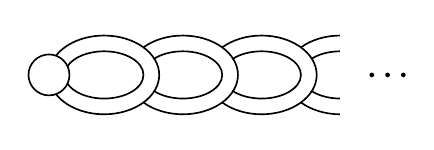
\begin{tikzpicture}[line width=.6, baseline=(base.base)]
    \draw (0,0) circle (.26);
    \draw (1.4,0) arc (0 : 151 : .7 and .5);
    \draw (1.4,0) arc (0 : -151 : .7 and .5);
    \draw (1.2,0) arc (0 : 159 : .5 and .3);
    \draw (1.2,0) arc (0 : -159 : .5 and .3);
    \draw (2.4,0) arc (0 : 136 : .7 and .5);
    \draw (2.4,0) arc (0 : -136 : .7 and .5);
    \draw (2.2,0) arc (0 : 138 : .5 and .3);
    \draw (2.2,0) arc (0 : -138 : .5 and .3);
    \draw (3.4,0) arc (0 : 136 : .7 and .5);
    \draw (3.4,0) arc (0 : -136 : .7 and .5);
    \draw (3.2,0) arc (0 : 138 : .5 and .3);
    \draw (3.2,0) arc (0 : -138 : .5 and .3);
    \draw (4.4,0) arc (0 : 136 : .7 and .5);
    \draw (4.4,0) arc (0 : -136 : .7 and .5);
    \draw (4.2,0) arc (0 : 138 : .5 and .3);
    \draw (4.2,0) arc (0 : -138 : .5 and .3);
    \fill[white] (3.7,.6) rectangle (4.5,-.6);
    \fill (4.1,0) circle (.03);
    \fill (4.3,0) circle (.03);
    \fill (4.5,0) circle (.03);
    \node (base) at (0,-.1) {};
\end{tikzpicture}
\qquad\Longrightarrow\qquad
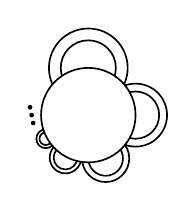
\begin{tikzpicture}[line width=.6, baseline=(base.base)]
    \draw[fill=white] (0,.6) circle (.5);
    \draw[fill=white] (0,.6) circle (.35);
    \draw[fill=white] (.6,0) circle (.4);
    \draw[fill=white] (.6,0) circle (.3);
    \draw[fill=white] (.22,-.55) circle (.3);
    \draw[fill=white] (.22,-.55) circle (.22);
    \draw[fill=white] (-.29,-.54) circle (.2);
    \draw[fill=white] (-.29,-.54) circle (.15);
    \draw[fill=white] (-.54,-.3) circle (.12);
    \draw[fill=white] (-.54,-.3) circle (.08);
    \draw[fill=white] (0,0) circle (.6);
    \fill (-.7, -.1) circle (.03);
    \fill (-.72, 0) circle (.03);
    \fill (-.74, .1) circle (.03);
    \node (base) at (0,-.1) {};
\end{tikzpicture} \]

As before, two relative handlebodies are \term{similar},
if the pairs $(N,A)$ are diffeomorphic as pairs of manifolds,
and for every $\lambda$, they have the same number (possibly infinite)
of $\lambda$-handles.
A relative handlebody is \term{good},
if every $\lambda$-handle is attached on handles of type $<\lambda$, or on $A$.

The proof will be given in \S\ref{sec-proofs}.

The cancellation theorem is also true,
with some modifications.

\begin{theorem}[Cancellation] \label{thm-cancel-weak}
    If a weak handlebody has a collection of pairs of handles
    satisfying the condition for cancellation,
    then these pairs can be cancelled simultaneously.
\end{theorem}

\[ 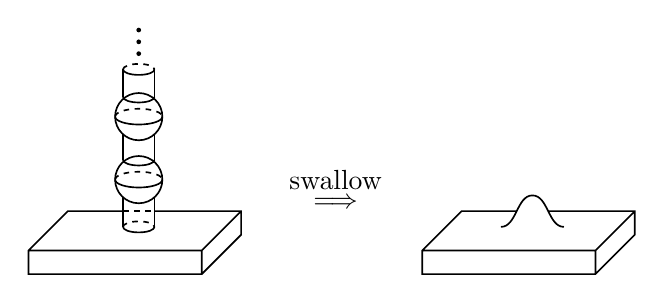
\begin{tikzpicture}[line width=.6]
    \tikzstyle{dp}=[dash pattern=on 2pt off 2pt]
    
    \draw (-.2,.2) -- (-.9,.2) -- (-1.4,-.3) -- (-1.4,-.6) -- (.8,-.6) -- (1.3,-.1) -- (1.3,.2) -- (.2,.2)
          (-1.4,-.3) -- (.8,-.3) -- (1.3,.2)
          (.8,-.3) -- (.8,-.6);
    \draw[dp] (-.2,.2) -- (.2,.2);

    \draw[dp] (-.2,0) arc (180 : 0 : .2 and .07);
    \draw (-.2,0) arc (180 : 360 : .2 and .07);
    \draw (-.2,0) -- (-.2,.38) (.2,0) -- (.2,.38);

    \draw (0,.6) circle (.3);
    \draw[dp] (-.3,.6) arc (180 : 0 : .3 and .1);
    \draw (-.3,.6) arc (180 : 360 : .3 and .1);

    \draw (-.2,.85) arc (180 : 360 : .2 and .07);
    \draw (-.2,.85) -- (-.2,1.18) (.2,.85) -- (.2,1.18);

    \draw (0,1.4) circle (.3);
    \draw[dp] (-.3,1.4) arc (180 : 0 : .3 and .1);
    \draw (-.3,1.4) arc (180 : 360 : .3 and .1);

    \draw (-.2,1.65) arc (180 : 360 : .2 and .07);
    \draw (-.2,1.65) -- (-.2,2) (.2,1.65) -- (.2,2);
    \draw (-.2,2) arc (180 : 360 : .2 and .07);
    \draw[dp] (-.2,2) arc (180 : 0 : .2 and .07);

    \fill (0,2.2) circle (.03);
    \fill (0,2.35) circle (.03);
    \fill (0,2.5) circle (.03);

    \node at (2.5,.3) {\text{$\Longrightarrow$}};
    \node at (2.5,.6) {\text{swallow}};
    
    \draw (4.8,.2) -- (4.1,.2) -- (3.6,-.3) -- (3.6,-.6) -- (5.8,-.6) -- (6.3,-.1) -- (6.3,.2) -- (5.2,.2)
          (3.6,-.3) -- (5.8,-.3) -- (6.3,.2)
          (5.8,-.3) -- (5.8,-.6);
    \draw (4.6,0) .. controls (4.8,0) and (4.8,.4) .. (5,.4)
                  .. controls (5.2,.4) and (5.2,0) .. (5.4,0);
\end{tikzpicture} \]

Precisely, \term{cancellation} means that the original handlebody is
diffeomorphic to a new handlebody, with the number of handles cut down.

A more precise formulation and the proof 
will be given as (\ref{thm:cancel-infinite}).
